\documentclass[14pt]{extbook}
\usepackage{multicol, enumerate, enumitem, hyperref, color, soul, setspace, parskip, fancyhdr} %General Packages
\usepackage{amssymb, amsthm, amsmath, latexsym, units, mathtools} %Math Packages
\everymath{\displaystyle} %All math in Display Style
% Packages with additional options
\usepackage[headsep=0.5cm,headheight=12pt, left=1 in,right= 1 in,top= 1 in,bottom= 1 in]{geometry}
\usepackage[usenames,dvipsnames]{xcolor}
\usepackage{dashrule}  % Package to use the command below to create lines between items
\newcommand{\litem}[1]{\item#1\hspace*{-1cm}\rule{\textwidth}{0.4pt}}
\pagestyle{fancy}
\lhead{Progress Quiz 5}
\chead{}
\rhead{Version C}
\lfoot{8497-6012}
\cfoot{}
\rfoot{Summer C 2021}
\begin{document}

\begin{enumerate}
\litem{
Solve the rational equation below. Then, choose the interval(s) that the solution(s) belongs to.\[ \frac{5}{7x + 6} + -7 = \frac{-6}{-28x -24} \]\begin{enumerate}[label=\Alph*.]
\item \( x_1 \in [-1.4, -0.7] \text{ and } x_2 \in [0.1,1.6] \)
\item \( \text{All solutions lead to invalid or complex values in the equation.} \)
\item \( x_1 \in [-1.4, -0.7] \text{ and } x_2 \in [-2,0.3] \)
\item \( x \in [-1.79,1.21] \)
\item \( x \in [0.7,2] \)

\end{enumerate} }
\litem{
Choose the equation of the function graphed below.
\begin{center}
    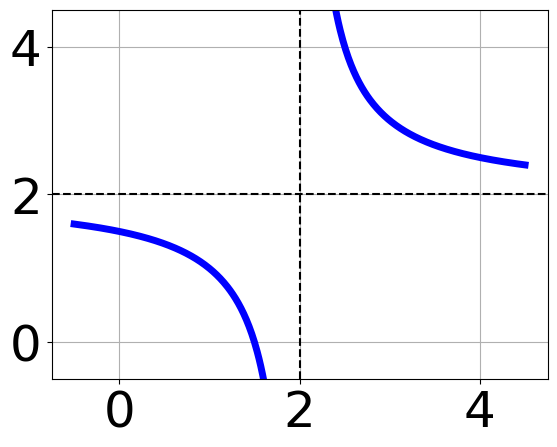
\includegraphics[width=0.5\textwidth]{../Figures/rationalGraphToEquationC.png}
\end{center}
\begin{enumerate}[label=\Alph*.]
\item \( f(x) = \frac{1}{x - 2} + 2 \)
\item \( f(x) = \frac{1}{(x - 2)^2} + 2 \)
\item \( f(x) = \frac{-1}{x + 2} + 2 \)
\item \( f(x) = \frac{-1}{(x + 2)^2} + 2 \)
\item \( \text{None of the above} \)

\end{enumerate} }
\litem{
Choose the equation of the function graphed below.
\begin{center}
    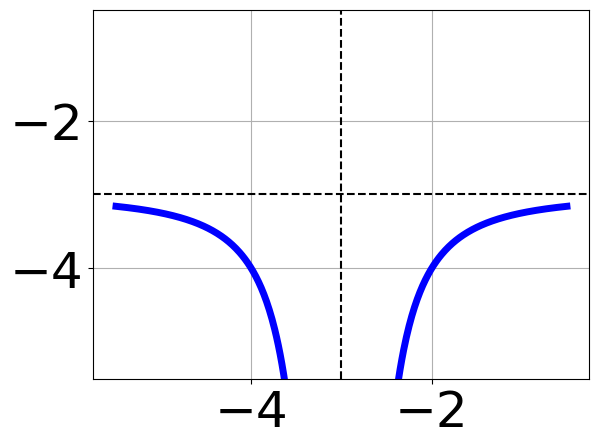
\includegraphics[width=0.5\textwidth]{../Figures/rationalGraphToEquationCopyC.png}
\end{center}
\begin{enumerate}[label=\Alph*.]
\item \( f(x) = \frac{-1}{x + 3} - 3 \)
\item \( f(x) = \frac{1}{(x - 3)^2} - 3 \)
\item \( f(x) = \frac{1}{x - 3} - 3 \)
\item \( f(x) = \frac{-1}{(x + 3)^2} - 3 \)
\item \( \text{None of the above} \)

\end{enumerate} }
\litem{
Choose the graph of the equation below.\[ f(x) = \frac{1}{(x + 1)^2} - 2 \]\begin{enumerate}[label=\Alph*.]
\begin{multicols}{2}\item 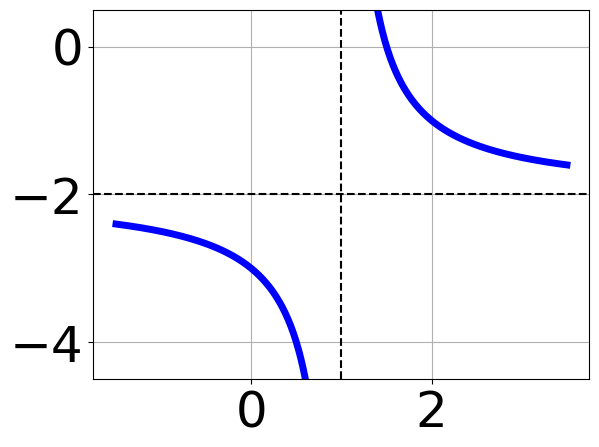
\includegraphics[width = 0.3\textwidth]{../Figures/rationalEquationToGraphCopyAC.png}\item 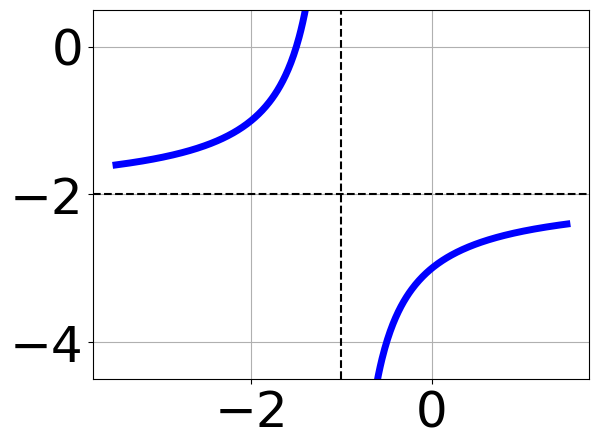
\includegraphics[width = 0.3\textwidth]{../Figures/rationalEquationToGraphCopyBC.png}\item 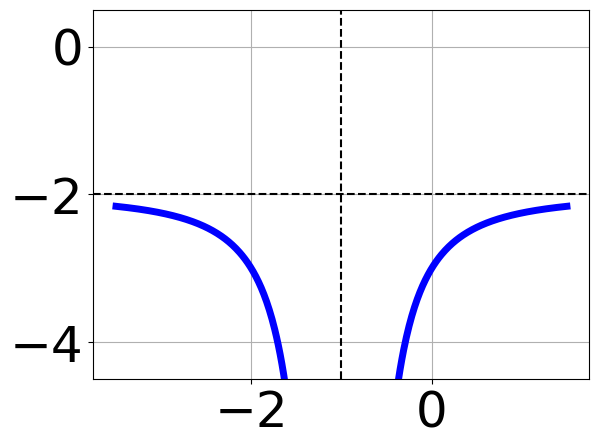
\includegraphics[width = 0.3\textwidth]{../Figures/rationalEquationToGraphCopyCC.png}\item 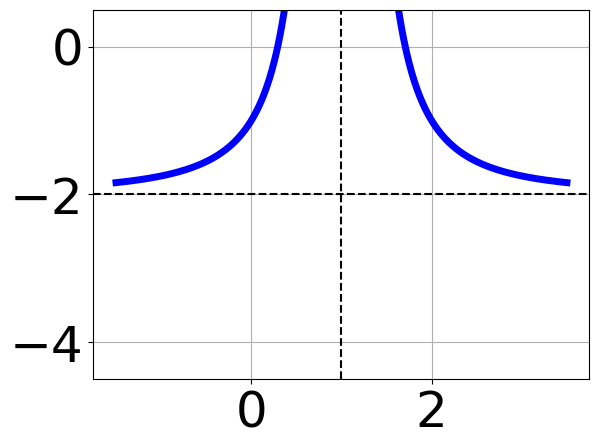
\includegraphics[width = 0.3\textwidth]{../Figures/rationalEquationToGraphCopyDC.png}\end{multicols}\item None of the above.
\end{enumerate} }
\litem{
Solve the rational equation below. Then, choose the interval(s) that the solution(s) belongs to.\[ \frac{-2x}{3x -2} + \frac{-6x^{2}}{6x^{2} +11 x -10} = \frac{-4}{2x + 5} \]\begin{enumerate}[label=\Alph*.]
\item \( \text{All solutions lead to invalid or complex values in the equation.} \)
\item \( x \in [0.65,0.68] \)
\item \( x \in [-2.54,-2.47] \)
\item \( x_1 \in [-2.6, -2.56] \text{ and } x_2 \in [1.56,2.56] \)
\item \( x_1 \in [0.65, 0.68] \text{ and } x_2 \in [-3.5,-1.5] \)

\end{enumerate} }
\litem{
Solve the rational equation below. Then, choose the interval(s) that the solution(s) belongs to.\[ \frac{-3x}{7x + 6} + \frac{-2x^{2}}{-28x^{2} -10 x + 12} = \frac{5}{-4x + 2} \]\begin{enumerate}[label=\Alph*.]
\item \( x_1 \in [-0.99, -0.27] \text{ and } x_2 \in [2.73,11.73] \)
\item \( \text{All solutions lead to invalid or complex values in the equation.} \)
\item \( x \in [0.36,0.75] \)
\item \( x \in [4.07,5.47] \)
\item \( x_1 \in [-0.99, -0.27] \text{ and } x_2 \in [-2.86,2.14] \)

\end{enumerate} }
\litem{
Determine the domain of the function below.\[ f(x) = \frac{6}{18x^{2} -6 x -24} \]\begin{enumerate}[label=\Alph*.]
\item \( \text{All Real numbers except } x = a, \text{ where } a \in [-3, 1] \)
\item \( \text{All Real numbers except } x = a \text{ and } x = b, \text{ where } a \in [-36, -35] \text{ and } b \in [12, 13] \)
\item \( \text{All Real numbers.} \)
\item \( \text{All Real numbers except } x = a, \text{ where } a \in [-36, -35] \)
\item \( \text{All Real numbers except } x = a \text{ and } x = b, \text{ where } a \in [-3, 1] \text{ and } b \in [0.33, 6.33] \)

\end{enumerate} }
\litem{
Determine the domain of the function below.\[ f(x) = \frac{3}{16x^{2} +8 x -24} \]\begin{enumerate}[label=\Alph*.]
\item \( \text{All Real numbers except } x = a \text{ and } x = b, \text{ where } a \in [-25.9, -22.9] \text{ and } b \in [14.9, 16.3] \)
\item \( \text{All Real numbers except } x = a \text{ and } x = b, \text{ where } a \in [-2.5, -0.7] \text{ and } b \in [-0.5, 1.4] \)
\item \( \text{All Real numbers except } x = a, \text{ where } a \in [-2.5, -0.7] \)
\item \( \text{All Real numbers except } x = a, \text{ where } a \in [-25.9, -22.9] \)
\item \( \text{All Real numbers.} \)

\end{enumerate} }
\litem{
Choose the graph of the equation below.\[ f(x) = \frac{-1}{x - 3} - 3 \]\begin{enumerate}[label=\Alph*.]
\begin{multicols}{2}\item 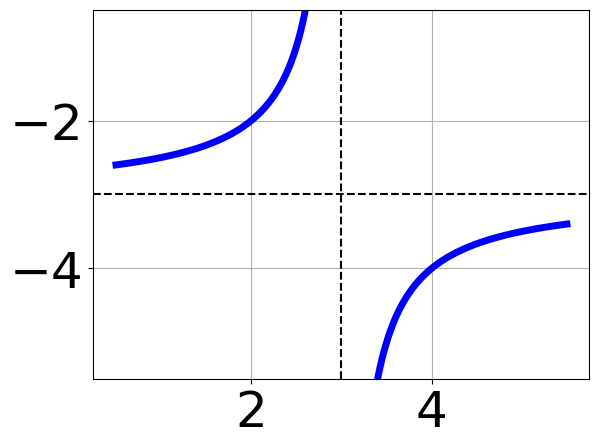
\includegraphics[width = 0.3\textwidth]{../Figures/rationalEquationToGraphAC.png}\item 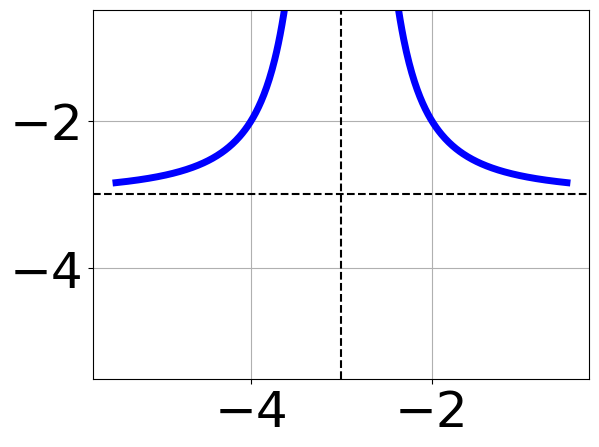
\includegraphics[width = 0.3\textwidth]{../Figures/rationalEquationToGraphBC.png}\item 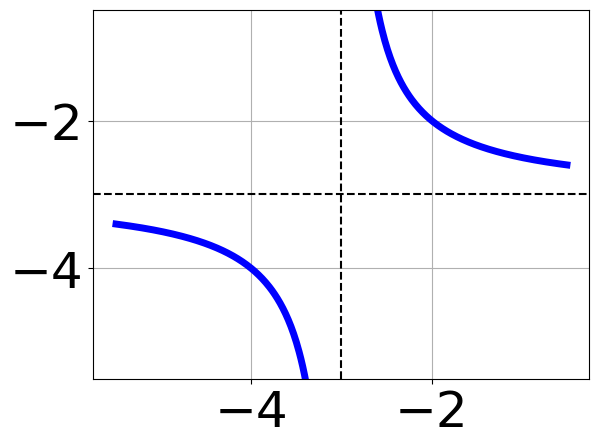
\includegraphics[width = 0.3\textwidth]{../Figures/rationalEquationToGraphCC.png}\item 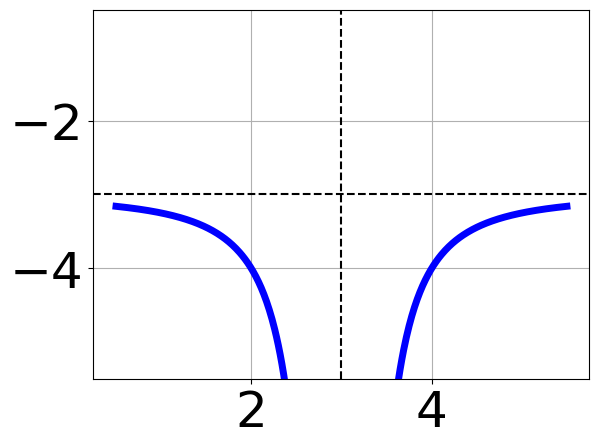
\includegraphics[width = 0.3\textwidth]{../Figures/rationalEquationToGraphDC.png}\end{multicols}\item None of the above.
\end{enumerate} }
\litem{
Solve the rational equation below. Then, choose the interval(s) that the solution(s) belongs to.\[ \frac{88}{88x + 55} + 1 = \frac{88}{88x + 55} \]\begin{enumerate}[label=\Alph*.]
\item \( \text{All solutions lead to invalid or complex values in the equation.} \)
\item \( x \in [-0.62,0.38] \)
\item \( x_1 \in [-1.62, 0.38] \text{ and } x_2 \in [-1.62,0.38] \)
\item \( x_1 \in [-1.62, 0.38] \text{ and } x_2 \in [0.62,1.62] \)
\item \( x \in [-0.38,2.62] \)

\end{enumerate} }
\end{enumerate}

\end{document}